\documentclass[bigger]{beamer}
%\documentclass[handout]{beamer}
\setbeamertemplate{bibliography item}{}
\usepackage[utf8]{inputenc}
\usepackage[english]{babel}
\usepackage{multirow}
\usepackage{synttree}
\usepackage{booktabs}
\usepackage[backend=bibtex,natbib,style=authoryear]{biblatex}
\usetheme{Warsaw}
%\usefonttheme[onlylarge]{structuresmallcapsserif}
\newcommand{\wigegraph}[1]{\begin{figure}[h]
\centering\includegraphics[width=\textwidth]{#1}\end{figure}}
% Ez most valamiert besz.rt, ugyhogy kikommentalom:
%\AtBeginSection[]{\frame{\frametitle{Outline}\tableofcontents[current]}}

\AtBeginPart{\frame{\partpage}} 

\usepackage{tikz}
\usepackage{tikz-qtree}
\usepackage{xspace}

\bibliography{ml}

\newcommand{\defl}{\texttt{dep\_to\_4lang}\xspace}
\newcommand{\difl}{\texttt{dict\_to\_4lang}\xspace}
\newcommand{\tfl}{\texttt{text\_to\_4lang}\xspace}
\newcommand{\tefl}{\texttt{text\_to\_4lang}\xspace}
\newcommand{\fl}{\texttt{4lang}\xspace}

\newcommand{\edge}[3]{\texttt{#1}~$\xrightarrow#2$~\texttt{#3}}
\newcommand{\twoedges}[4]{\texttt{#1}~$\overset{#2}{\underset{#3}{\rightleftharpoons}}$~\texttt{#4}}
\newcommand{\bin}[3]{
    \texttt{#2}~$\xleftarrow1$~\texttt{#1}~$\xrightarrow2$~\texttt{#3}}

\newcommand{\todo}[1]{\textbf{TODO: #1}}

%\usepackage{apacite}
%\let\cite\shortcite  % to get "et al." for more than two authors
%\let\citeA\shortciteA
\begin{document}

\title{Szemantikai elemz\'es gr\'af-transzform\'aci\'okkal}
\author{Kov\'acs \'Ad\'am \\ G\'emes Kinga}
\institute{\texttt{kovacs.adam@aut.bme.hu}, \texttt{kinga.andrea.gemes@gmail.com}}

\date{Országos Tudományos Diákköri Konferencia\\2019.04.17.}

%-----------------------

\begin{frame} 

\titlepage 

\end{frame} 
%----------------------

%-----------------------

\begin{frame} 

    \frametitle{Kontribúciónk} 
    \begin{itemize}
        \pause \item Gráf alapú szemantikai modellek definiálása
        \pause \item Modelleink kiértékelése a gépi szövegértés feladaton
        \pause \item Modellünk beépítése egy state-of-the-art rendszerbe
        \pause \item Előzetes eredmények szerint a rendszeren javulást hozva
    \end{itemize}

\end{frame} 

%-----------------------
\begin{frame}
	\frametitle{A gépi szövegértés feladat \citep{Chen:2018, Wang:2018}}
	\textbf{Sz\"oveg:} "Today we decided to paint the extra room in our house. Were going to have visitor coming next month so hopefully the painting ain't that smelly anymore. I made sure that the wall is clean and clear of all the nuisance. We already bought the pain and we decided the new wall pain is sky blue. My husband is putting newspaper on the floor to avoid any spill on our floor/carpet....." \\
	\textbf{Kérdés:} "Did anyone help him?" \\
	\textbf{1. v\'alaszlehet\H{o}s\'eg:} "It was the narrator and her husband" \\
	\textbf{2. v\'alaszlehet\H{o}s\'eg:} "No, he worked alone."
\end{frame}

%---------------------

\begin{frame}
	\frametitle{A gépi szövegértés feladat \citep{Chen:2018, Wang:2018}}
	\begin{columns}
		\begin{column}{0.6\textwidth}
			\begin{itemize}
				\pause \item \textbf{2018-as Semeval Task}
				\begin{itemize}
					\item \textit{Machine comprehension using commonsense knowledge}
				\end{itemize}
				\pause \item Rövid szövegekből egyszerű feleletválasztós kérdések
			\end{itemize}
		\end{column}
		\begin{column}{0.5\textwidth}
			\begin{itemize}
				\pause \item Két legjobb rendszer
				\begin{itemize}
					\item \texttt{HFL-RC}
					\item \texttt{Yuanfudao}
				\end{itemize}
				\pause \item \textbf{MCScript}
				\begin{itemize}
					\item tanító és teszt adat
				\end{itemize}
			\end{itemize}
		\end{column}
	\end{columns}
	
\end{frame}

%-----------------------
{
\setbeamerfont{frametitle}{size=\small}

\begin{frame}
    \frametitle{\fl: a formalizmus \citep{Kornai:2010,Kornai:2015a}}
\pause Irányított fogalmi gráfok, 3 típusú él:
\begin{itemize}
    \pause \item 0 típusú él
        \begin{itemize}
            \pause \item tulajdonság: \texttt{dog}~$\xrightarrow0$~\texttt{large}
            \pause \item \texttt{IS\_A} reláció (hipernima): \texttt{dog}~$\xrightarrow0$~\texttt{mammal}
            \pause \item állítmány: \texttt{dog}~$\xrightarrow0$~\texttt{bark}
        \end{itemize}
    \pause \item 1- és 2-es él bináris állítmányt köt össze az argumentumokkal.
\end{itemize}
\pause \begin{figure}
\centering
    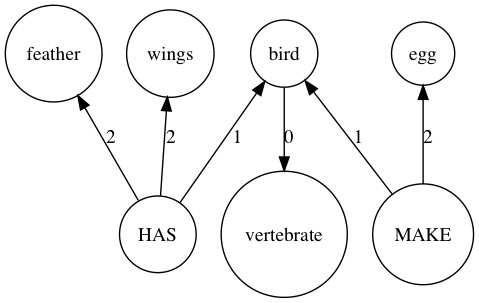
\includegraphics[scale=0.4]{pics/bird.jpg}
\end{figure}
\end{frame}
}
%-----------------------
\begin{frame}
\frametitle{A 4lang szolgáltatás}
		\begin{itemize}
			\pause \item Éles service a \tefl modulra építve
			\pause \item Magasan automatizált gráfgenerálás
			\pause \item Online demo
			\begin{itemize}
				 \item \url{http://4lang.hlt.bme.hu}
			\end{itemize}
			\pause \item Github
			\begin{itemize}
				\item \url{https://github.com/adaamko/4lang}
			\end{itemize}
		\end{itemize}

\end{frame}
%-----------------------
%-----------------------
\begin{frame}
\frametitle{A 4lang szolgáltatás}
\begin{columns}
	\begin{column}{0.3\textwidth}
		\pause My poor wife!
		\pause 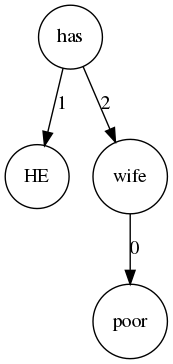
\includegraphics[scale=0.4]{pics/wifepoor.png}
	\end{column}
	\begin{column}{0.4\textwidth}
		I feel bad for my wife!
		\pause 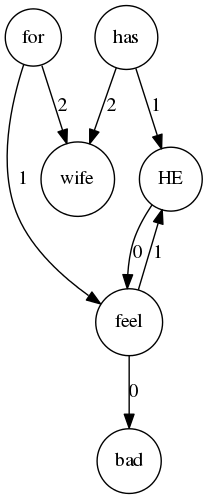
\includegraphics[scale=0.4]{pics/feelbad.png}
	\end{column}
\end{columns}

\end{frame}
%-----------------------
\begin{frame}
\frametitle{Definiált metrikáink}
\begin{columns}
	\begin{column}{0.5\textwidth}
		\begin{itemize}
			\pause \item \textbf{Cél}
			\begin{itemize}
				\item egy állítás következik-e egy feltevésből?
			\end{itemize}
			\pause \item \textbf{Megvalósítás}
			\begin{itemize}
				\item Gráfok hasonlósága
				\item Mikor hasonló két gráf?
			\end{itemize}
		\end{itemize}
	\end{column}
	\begin{column}{0.5\textwidth}
		\begin{itemize}
			\pause \item My poor wife! (G1)
			\pause \item I feel bad for my wife! (G2)
			\pause \item \[\frac{|E(G_1)\cap E(G_2)|}{|E(G_2)|}\]			
		\end{itemize}
	\end{column}
\end{columns}

\end{frame}
%-----------------------
\begin{frame}
\frametitle{Kiterjesztett gráfok, az "expand" funkció}
\begin{columns}
	\begin{column}{0.1\textwidth}
		\pause 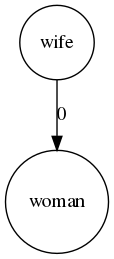
\includegraphics[scale=0.4]{pics/wife.png}
	\end{column}
	\begin{column}{0.1\textwidth}
	\pause \[\Rightarrow\]
	\end{column}
	\begin{column}{0.2\textwidth}
		\pause 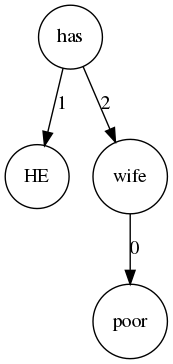
\includegraphics[scale=0.4]{pics/wifepoor.png}
	\end{column}
	\begin{column}{0.1\textwidth}
		\pause \[\Rightarrow\]
	\end{column}
	\begin{column}{0.3\textwidth}
	\pause 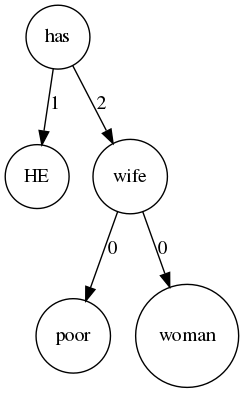
\includegraphics[scale=0.4]{pics/wifeexp.png}
	\end{column}
\end{columns}
\end{frame}

%--------------------------------------------

\begin{frame}
    \frametitle{Baseline}
    \begin{figure}
        \centering
        \small
            \begin{itemize}
				\item Minden kérdés válasz párhoz mergelt gráf
				\item A "jobban" hasonló lesz a helyes válasz
				\item \textbf{68,3} accuracy score
			\end{itemize}
            \begin{columns}
				\begin{column}{0.2\textwidth}
					\pause 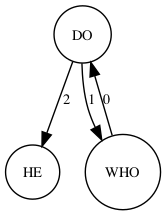
\includegraphics[scale=0.5]{pics/didit.png}
				\end{column}
				\begin{column}{0.2\textwidth}
				\pause \[\Rightarrow\]
				\end{column}
				\begin{column}{0.2\textwidth}
					\pause 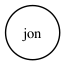
\includegraphics[scale=0.5]{pics/jon.png}
				\end{column}
				\begin{column}{0.2\textwidth}
					\pause \[\Rightarrow\]
				\end{column}
				\begin{column}{0.3\textwidth}
				\pause 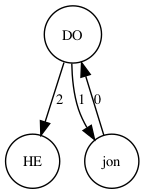
\includegraphics[scale=0.5]{pics/jondid.png}
				\end{column}
			\end{columns}
        \label{fig:method}
        \end{figure}
\end{frame}

%-----------------------

\begin{frame}
	\frametitle{M\'ely tanul\'as}
	\begin{itemize}
		\pause \item Elterjedt m\'odszer
		\pause \item Term\'eszetes nyelvfeldolgoz\'asban \'elenj\'ar\'o
		\pause \item RNN a szekvenci\'akat eset\'en a leghat\'ekonyabb
		\begin{itemize}
			\pause \item LSTM
			\pause \item Attention
		\end{itemize}
	\end{itemize}
\end{frame}

%-----------------------

\begin{frame}
	\frametitle{Yuanfudao rendszer}
	\begin{figure}[h!]
		\centering
		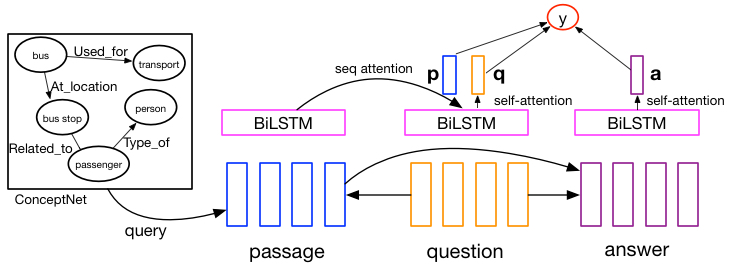
\includegraphics[scale=0.4]{pics/TriAN.jpg}
		\caption{A rendszer strukt\'ur\'aja}
		\label{fig:dnn}
	\end{figure}
\end{frame}
%-----------------------
\begin{frame}
	\frametitle{M\'odos\'it\'asok}
	\begin{itemize}
		\pause \item 4lang hasonl\'os\'ag sz\'am\'it\'as a szavak k\"oz\"ott az el\H{o}feldolgoz\'as sor\'an
		\pause \item \'Uj embedding r\'eteg a 4lang hasonl\'os\'agokhoz
		\pause \item Az RNN r\'eteg b\H{o}v\'it\'ese, hogy a megfelel\H{o} RNN-ek megkapj\'ak a 4lang embedding kimenet\'et
	\end{itemize}
\end{frame}


%-----------------------

\begin{frame}
	\frametitle{Eredm\'enyek}
	\begin{table}[h!]
		\centering
		\begin{tabular}{ | l | c | r | }
			\hline
			modell & dev adat & teszt adat \\ \hline \hline el\H{o}tan\'itott TriAN, ConceptNet n\'elk\"ul & 83.7\% & 81.9\% \\ \hline
			el\H{o}tan\'itott TriAN, ConceptNettel & 82.5\% & 80.3\% \\ \hline
			el\H{o}tan\'itott TriAN, 4langgal & 84.2\% & 81.5\% \\ \hline
			\textbf{el\H{o}tan\'itott TriAN, mindkett\H{o}vel} & \textbf{83.4\%} & \textbf{82.9\%} \\ \hline
			TriAN, ConceptNet n\'elk\"ul & 82.8\% & 80.2\% \\ \hline
			TriAN, ConceptNettel & 82.7\% & 80.5\% \\ \hline
			TriAN, 4langgal & 83.2\% & 80.9\% \\ \hline
			TriAN, mindkett\H{o}vel & 83.1\% & 80.8\% \\ \hline
		\end{tabular}
		\caption{A \texttt{4lang} \'es a \texttt{ConceptNet} hat\'asa az eredm\'enyeken}
		\label{tabl:res}
	\end{table}
\end{frame}

%-----------------------
\begin{frame}
\frametitle{Összefoglalás}
	\begin{itemize}
	    \pause \item Automatizált módszer és metrikák hasonlóság mérésére.
	    \pause \item Erős baseline a gépi szövegértés feladatra
	    \pause \item Baseline módszerunk alkalmazása state-of-the-art rendszerben, kis javulást hozva
	    \pause \item A kód elérhető \url{https://github.com/adaamko/4lang}
	    \pause \item Éles Rest API és online demo \url{http://4lang.hlt.bme.hu}
	\end{itemize}

\end{frame}
%-----------------------
%-----------------------
\begin{frame}
    \frametitle{K\"osz\"onj\"uk a figyelmet!}
    \AtNextBibliography{\tiny}
    \printbibliography
\end{frame}
%-----------------------


\end{document}






